%!TEX root = ../paper.tex

\section{Evaluation}
\label{section:evaluation}

As part of our implementation, we needed a way to test our Pulsarcast system.
However we had a set of specific requirements that made our choice of tools
harder. We needed something that fulfilled the following:

\begin{itemize}
  \item Easily deploy and test different versions of our module.
  \item Run tests not only on Pulsarcast but also on IPFS' own pub-sub
    implementation.
  \item Able to extract relevant usage metrics.
  \item Simulate network constraints such as latency.
  \item Able to run locally but easily scalable to a large network.
  \item Can be controlled from a central point, while being able to interact
    with specific nodes in the system.
  \item Easy to create scripts for, so that we could automate as much of our
    test suite as possible.
\end{itemize}

Out of this list, a core principle that can be extracted is
reproducibility. Reproducibility allows us to run our testbed locally or in a
cloud service somewhere in the world and still expect the same behaviour and
results. Reproducibility is usually achieved through virtualisation mechanisms
that allow a certain workload to behave and act the same, whether we are
running it locally in our workstation or in a machine with different
specifications in the other end of the world. Nowadays this is most commonly
done through containerisation
techniques~\footnote{\url{https://www.freebsd.org/doc/handbook/jails.html}}~\footnote{\url{https://blog.jessfraz.com/post/containers-zones-jails-vms}}
with tools such as
Docker~\footnote{\url{https://www.docker.com/products/container-runtime}}, which we
used to create a containerised version of our module. To orchestrate our
containerised application we used Kubernetes~\footnote{\url{https://kubernetes.io/}},
an open source orchestration platform based on Google's learnings on running
containerised workloads at
scale~\footnote{\url{https://research.google/pubs/pub43438/}}, and one of the most
popular solutions in the field.

To aggregate, correlate and analyse metrics and logs we used Elasticsearch~\footnote{\url{https://www.elastic.co/products/elasticsearch}}, Beats~\footnote{\url{https://www.elastic.co/products/beats}}, Logstash~\footnote{\url{https://www.elastic.co/products/logstash}} and Kibana~\footnote{\url{https://www.elastic.co/products/kibana}}. In order to simulate abnormal network conditions we relied on Toxiproxy~\footnote{\url{http://toxiproxy.io}}, a TCP proxy that, programatically through an HTTP API, allowed us to inject multiple kinds of faults.

As we know it, Pulsarcast is just a module that applications can use to build
on top of. In order to test it we created a fork of JS
IPFS~\footnote{\url{https://github.com/jgantunes/js-ipfs}} where we integrated
Pulsarcast. This not only provided us with a command line interfaace (CLI) and
an HTTP API to interact with our system, but it also gave us direct access to
IPFS' own pub-sub module, Floodsub, to which we wanted to compare our module.

Figure \ref{fig:ipfs-testbed-and-metrics} provides an architectural overview of
our system. All of the projects and code we created for the testbed are
open
source~\footnote{\url{https://github.com/JGAntunes/helm-charts/tree/master/ipfs-testbed}}~\footnote{\url{https://github.com/JGAntunes/ipfs-testbed}}~\footnote{\url{https://github.com/JGAntunes/ipfs-testbed-cli}}.

\begin{figure}[!htb]
  \centering
  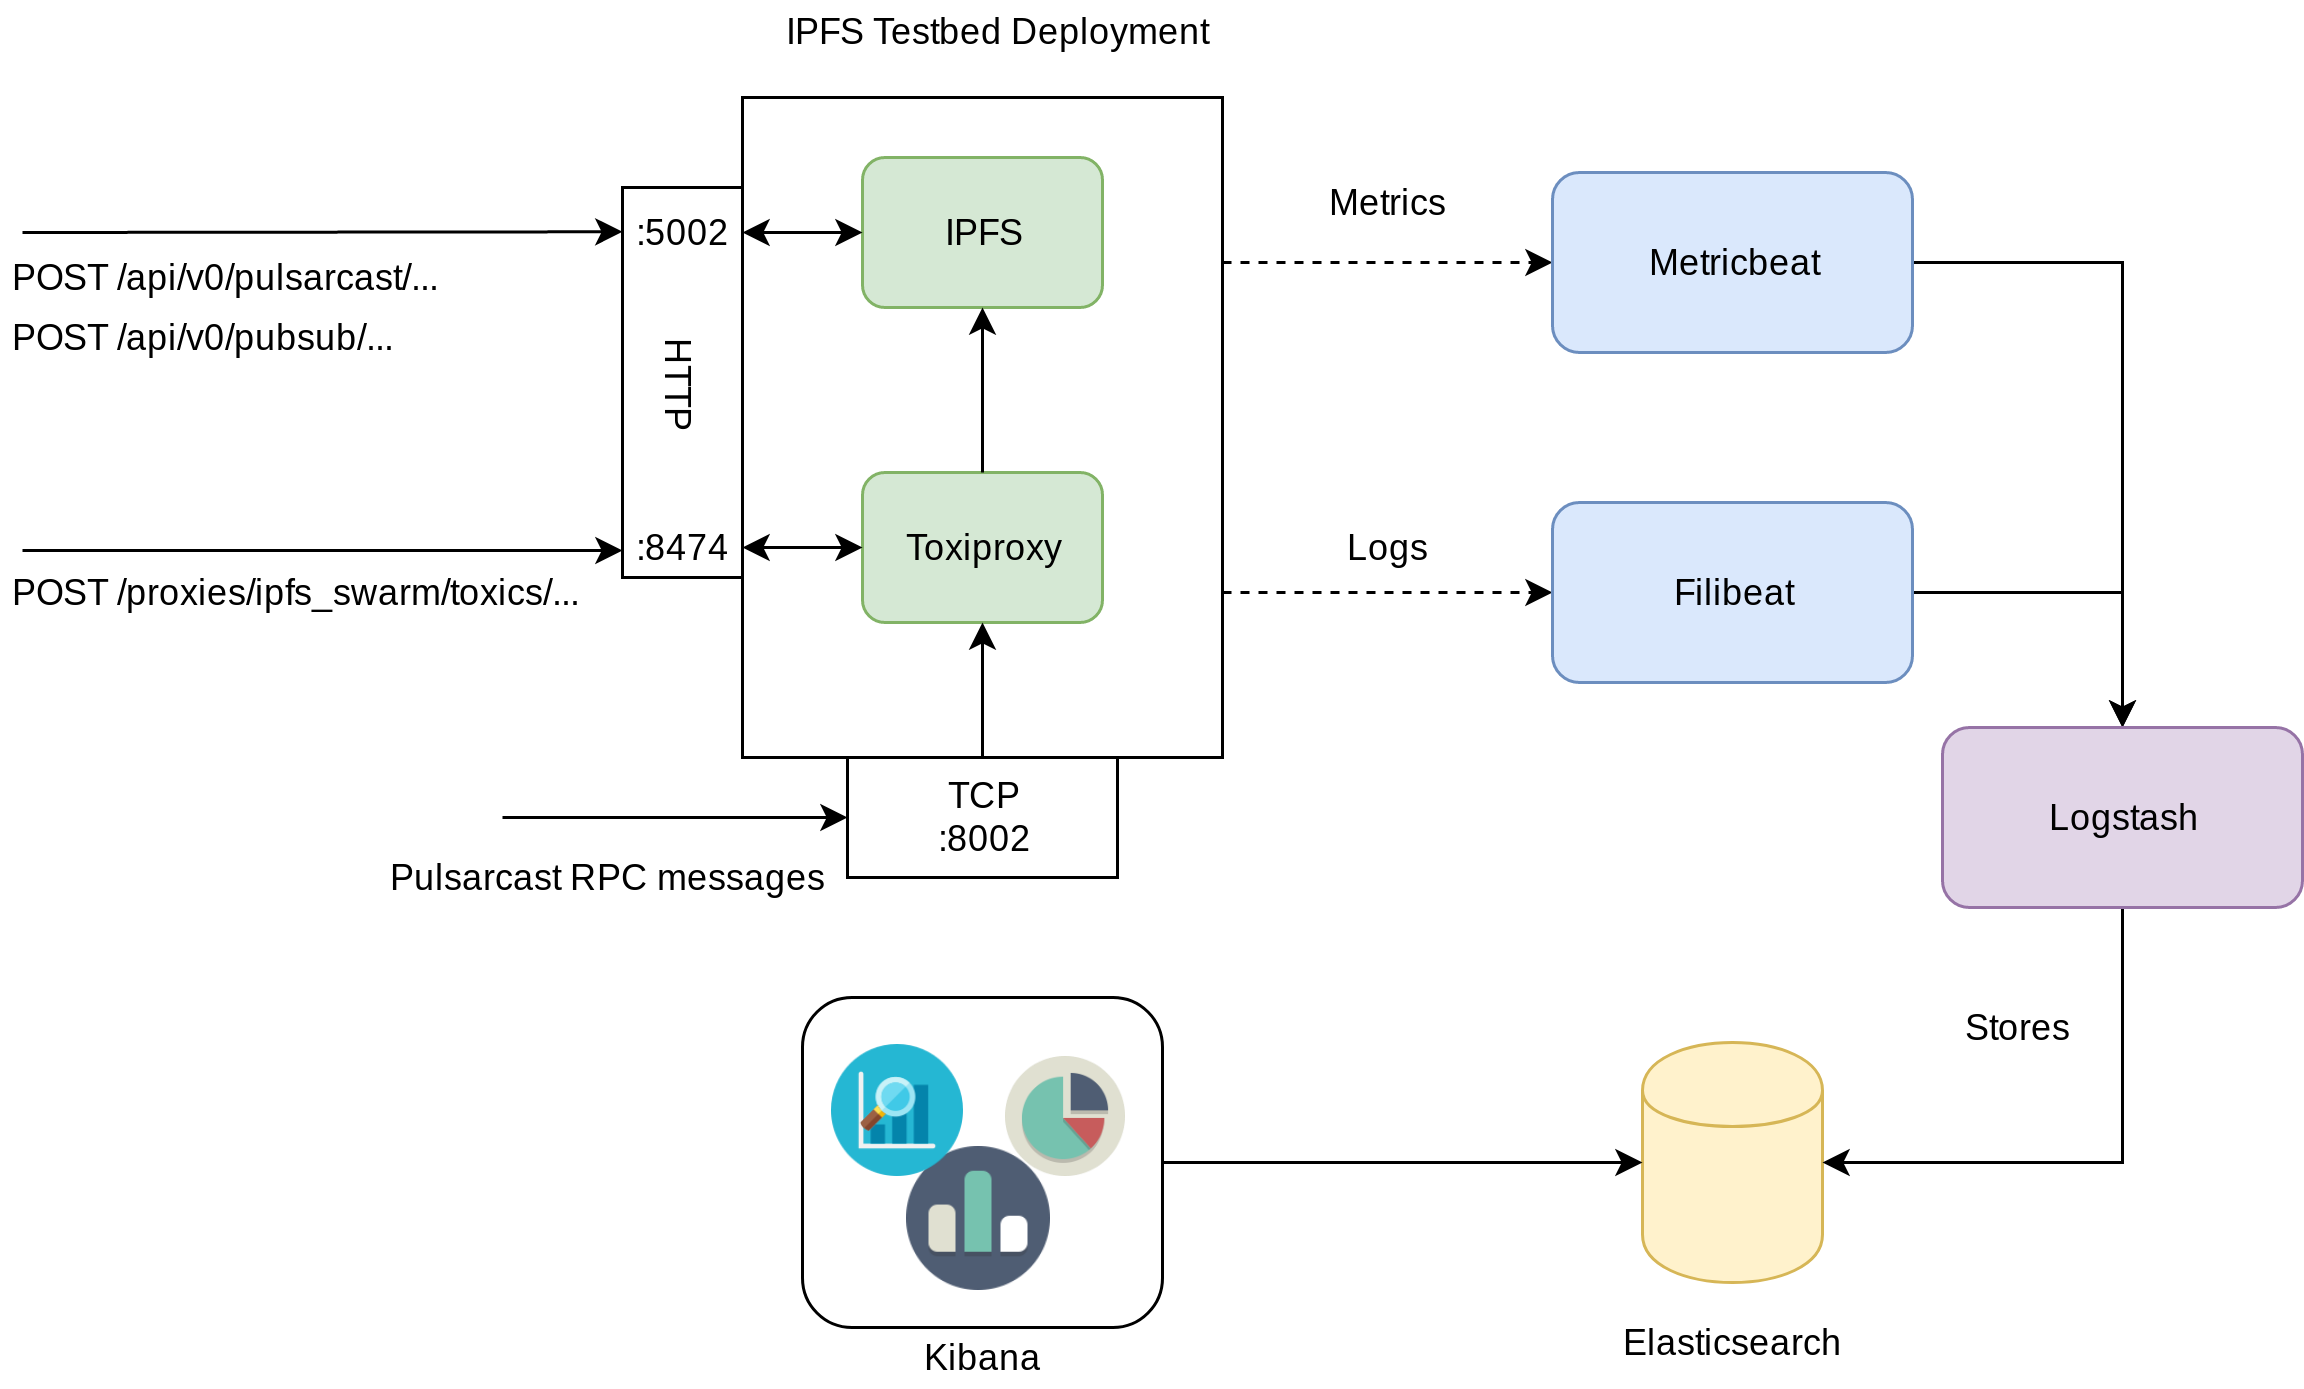
\includegraphics[width=0.45\textwidth]{img/ipfs-testbed-and-metrics.png}
  \caption{Overview of our ipfs-testbed deployment and our metrics/logs
  pipeline}
  \label{fig:ipfs-testbed-and-metrics}
\end{figure}

Our whole setup consisted of a total of 5 VMs~\footnote{Special thanks to
Microsoft and the Azure team for supporting our efforts and offer us free
credits} acting as Kubernetes Worker nodes, each with two vCPUs, 16 GiB of RAM
and 32 GiB of storage. In our cluster, besides other operational bits, we ran 3
Elasticsearch instances, 1 Logstash instance, 1 Kibana and a total of 100 IPFS
Testbed deployments (as described aboe). Because we wanted to avoid resource
starvation and to better take advantage of the Kubernetes scheduler, our
testbed deployments allocate 440 MiB of memory per deployment, each burstable
to a maximum of 500 MiB. During our whole test execution, periodic HTTP health
checks (part of the Kubernetes platform) make sure our deployments are working
accordingly.

To test our system accordingly, we wanted a dataset that could simulate a
real-life scenario as much as possible. We chose to use a dataset of
Reddit's~\footnote{\url{https://www.reddit.com/}} comments from
2007~\footnote{\url{http://academictorrents.com/details/7690f71ea949b868080401c749e878f98de34d3d}}~\footnote{\url{https://www.reddit.com/r/datasets/comments/3bxlg7/i_have_every_publicly_available_reddit_comment/}}
consisting of a sample of approximately 25000 comments in a total of 23 topics
(known as subreddits in the platform)~\footnote{\url{https://github.com/JGAntunes/pulsarcast-test-harness}}.

The following graphs give us a distribution analysis of events published per
topic (Figure \ref{fig:events-to-be-publisher-per-topic}), subscriptions per
topic (Figure \ref{fig:subscriptions-per-topic}) and subscription distribution
per nodes (Figure \ref{fig:subscription-distribution-per-node}). Given our
dataset choice, we aimed for a non-uniform subscription distribution per topic
and, as it would be expected in a real-world scenario, the distribution of
events follows a power law based on their popularity. 

\begin{figure}[!htb]
  \centering
  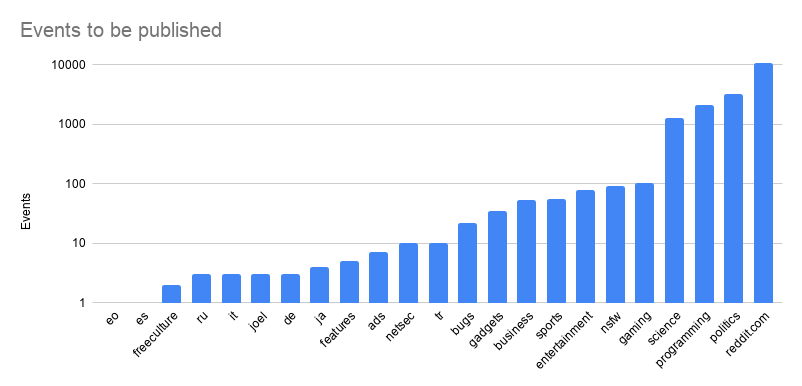
\includegraphics[width=0.35\textwidth]{img/events-to-be-publisher-per-topic.png}
  \caption{Event distribution per topic with log scale}
  \label{fig:events-to-be-publisher-per-topic}
\end{figure}

\begin{figure}[!htb]
  \centering
  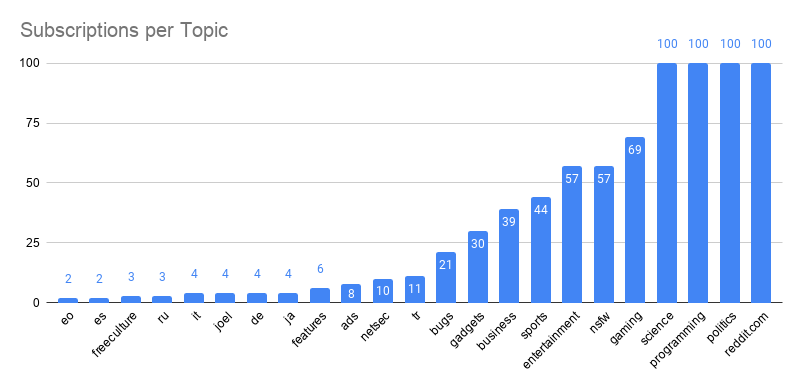
\includegraphics[width=0.35\textwidth]{img/subscriptions-per-topic.png}
  \caption{Subscription distribution per topic}
  \label{fig:subscriptions-per-topic}
\end{figure}

\begin{figure}[!htb]
  \centering
  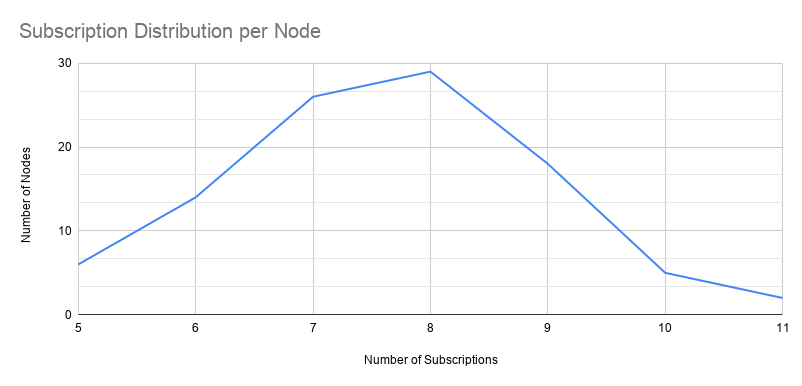
\includegraphics[width=0.4\textwidth]{img/subscription-distribution-per-node.png}
  \caption{Subscription distribution per number of nodes}
  \label{fig:subscription-distribution-per-node}
\end{figure}

For each execution, we look to extract two key groups of data: resource usage
data and QoS data. The following list describes these in more detail:

\begin{itemize}
  \item Resource usage as a total in the whole cluster, and per-node (95/99
  percentile and average)
  \begin{itemize}
    \item CPU Usage (CPU number)
    \item Memory Usage (GiB)
    \item Network Usage (MiB transmitted)
  \end{itemize}
  \item QoS
  \begin{itemize}
    \item Events published by topic and in total
    \item Events received by topic and in total
    \item Percentage of subscriptions fulfilled based on the number of events
    successfully published
    \item Percentage of subscriptions fulfilled based on the total number of events
    injected in the system
    \item Number of RPC messages sent per topic and in total
    \item Average, standard deviation and percentiles (99/95) of the number of RPC messages received and sent by each node
  \end{itemize}
\end{itemize}

We measure the subscription coverage (number of subscriptions fulfilled)
through two distinct metrics. The percentage of fulfillment having the number
of events effectively published as a reference and the percentage of
fulfillment having the total number of events injected into the system as
reference. Given Pulsarcast's nature, when an event is injected into the
system, depending on the topic configuration, it may need to be propagated
through the dissemination trees before being effectively published
(\emph{request to publish}). It also needs to be persisted in the DHT. Having
two different metrics allows us to better analyse and distinguish the different
behaviours of the system.

It is essential to keep in mind that some of the metrics under the QoS group
only make sense in Pulsarcast test runs, hence will be ignored when running the
baseline Floodsub solution.
